\documentclass[a4paper]{article}

%% Language and font encodings
\usepackage[english]{babel}
\usepackage[utf8x]{inputenc}
\usepackage[T1]{fontenc}

%% Sets page size and margins
\usepackage[a4paper,top=3cm,bottom=2cm,left=3cm,right=3cm,marginparwidth=1.75cm]{geometry}

%% Useful packages
\usepackage{amsmath}
\usepackage{graphicx}
\usepackage[colorinlistoftodos]{todonotes}
\usepackage[colorlinks=true, allcolors=blue]{hyperref}

\title{Actividad V}
\author{Jose Pablo Montaño de la Ree}
\date{Marzo 6,2018} 

\begin{document}
\maketitle


\section{Introduction}

En esta actividad, se continuo con lo ya creado u obtenido en la practica 4, donde se logro un archivo que contenia toda la informacion de 12 meses de ondeos de una estacion espesifica. Este archivo fue procesado para conservar solamente las fechas, PW y CAPE. despues este archivo fue limpiado usando las herramientas de emacs y la terminal para lograr un archivo que contuviese la informacion de 00Z, con los datos puestos en columnas de fecha, CAPE y PW, de la misma forma se obtuvo uno de 12Z.

\section{CAPE y PW}

CAPE, convective available potential energy o energia potencial convectiva disponible, se refiere a la cantidad de enerrgia que tendria una parcela de aire si se levantara cierta altura en direccion de la atmosfera. Esta medida se utuiliza para encontrar inestabilidad en la atmosfera, ya que esta se refiere a la fuerza boyante postiva de una parcela de aire, donde se coloca una capa de aire frio sobre uno caliente, haciendo que el caliente quiera subir. Esto tiene una alta importancia debido que  al elevarse las capas de aire se provocan tormentas con rayos. 
\linebreak

PW, precipitable water, o agua precipitable, se refiere a la cantidad de agua que hay en cierta columna de agua en la atmosfera. 

\section{Preparacion de los datos}

Se incio con un archivo que tenia toda la informacion de los 12 meses de lanzamientos. para limpiarlo, se escribio el siguiente comando en la termianl:

\begin{verbatim}

egrep -v 'PRES|hPa' df2017.csv | egrep '42867 |CAPE|Precip' > df2017CAPE_PW.csv

\end{verbatim}

Este comando tomo toda la informacion de CAPE, Precip y las fechas y las coloco en un nuevo archivo. Este aun tenia mucha informacion basura, informacion desordenada y le hacian falta comas.

Para eliminar la informacion inecesaria de cada renglon:


\begin{verbatim}

Se selleciono esa informacion con cntrl+w y se recoloco con cntrl+y. 
Despues se utilizo esc+shift+5 para iniciar querry replace. Se le 
proporcionaba la parte a remplazar con contrl+y y se le indicaba 
que lo reemplazara por nada para eliminarlo. Para confirmar la 
orden se escribio shift+1.


\end{verbatim}

Al quitar la informacion inecesaria y un procesos posterior se lograron columnas con la informacion, sin embargo jupyther aun no podia leerlo, pues necesitaba ciertas comas.

\begin{verbatim}

Para agregar informacion se indentificaron patrones de donde se tenain
que agregar comas o agregar espacios. Para esto se seleccionaba esa area
y se daba cntrl+w y se recoloco con cntrl+y. Despues se reutilizo querry
replace, dandole la informacion a remplazar por esta misma más una coma o
un espacio, quitandole un espacio etc.

\end{verbatim}

Despues se separaron los datos de 00Z y 12 Z usando egrep en la terminal de la siguiente forma.

\begin{verbatim}
Wolverine@ltsp70:~/Fisica Computacional/ActividadV$ grep 00Z df2017CAPE_PW.csv >df00Z.csv

Wolverine@ltsp70:~/Fisica Computacional/ActividadV$ grep 12Z df2017CAPE_PW.csv >df12Z.csv

\end{verbatim}

De esta forma se separo la informacion en dos archivos diferentes, donde despues se elimino las columnas de 00Z y 12Z, con el proceso mencionado en la seccion sobre eliminar informacion. 

\section{Analisis con pandas}

Para realizar el analisis de la informacion con pandas, se llamo estas bibliotecas yse hicieron unos cambios en las fechas leidas con pandas conlos siguientes procesos. 

\begin{verbatim}

import pandas as pd
import numpy as np
from datetime import datetime

# Leer archivo de datos
# Convertir la columna CAPE de objeto a número
df = pd.read_csv("ARCHIVO.csv", header=None, names=['Date', 'CAPE', 'PW'], sep = ",")
df.CAPE=pd.to_numeric(df.CAPE, errors='coerce')

# Convertir la cadena de caracteres 'Date' en variable temporal 'NDate'
df['Ndate'] = pd.to_datetime(df['Date'], format='%d %m %Y')
df['month'] = df['Ndate'].dt.month
df.head()



\end{verbatim}

Despues se procedio a realizar las graficas que se veran en la seccion de resultados. 

\section{Resultados}



\begin{figure}[h]
\centering
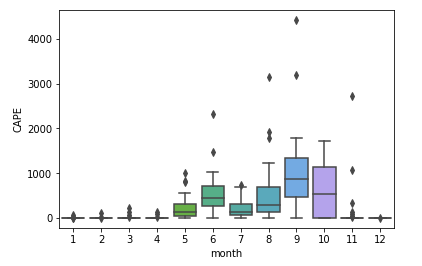
\includegraphics[width=0.3\textwidth]{1.png}
\caption{\label{fig:}Mes vs Convective Available Potential Energy OOZ}
\end{figure}


\begin{figure}[h]
\centering
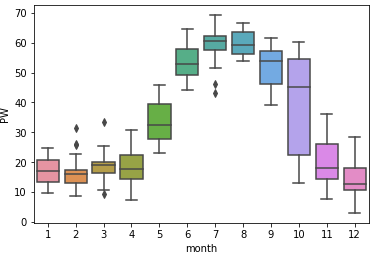
\includegraphics[width=0.3\textwidth]{2.png}
\caption{\label{fig:}Mes vs Agua precipitable OOZ}
\end{figure}

\begin{figure}[h]
\centering
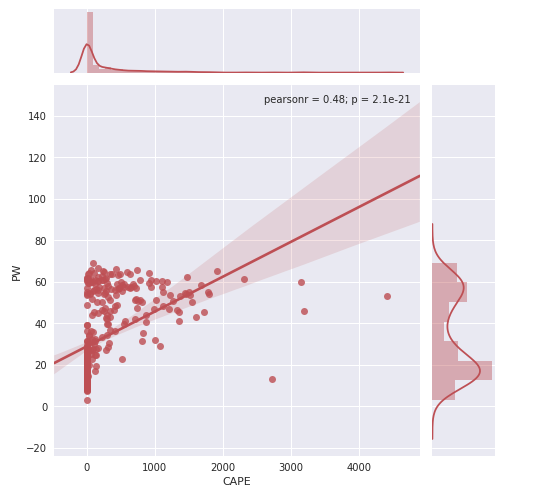
\includegraphics[width=0.3\textwidth]{3.png}
\caption{\label{fig:}Convective Available Potential Energy vs Agua Precipitable OOZ}
\end{figure}

\begin{figure}[h]
\centering
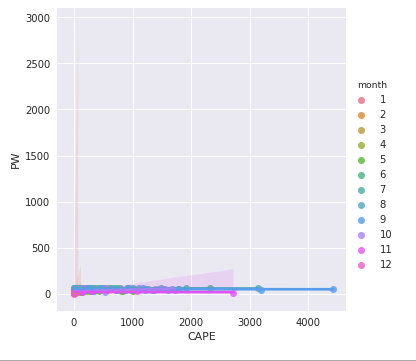
\includegraphics[width=0.3\textwidth]{4.png}
\caption{\label{fig:}Convective Available Potential Energy vs Agua Precipitable OOZ}
\end{figure}


\begin{figure}[h]
\centering
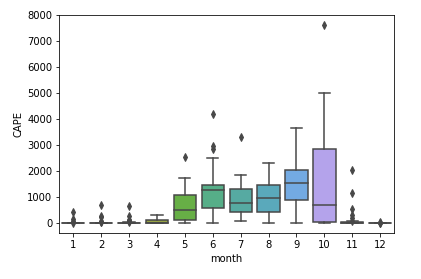
\includegraphics[width=0.3\textwidth]{5.png}
\caption{\label{fig:}Mes vs Convective Available Potential Energy 12Z}
\end{figure}

\begin{figure}[h]
\centering
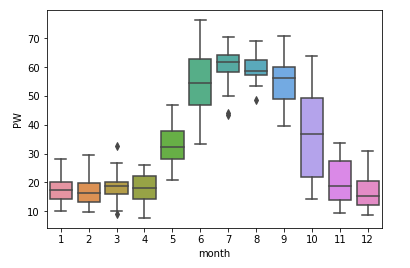
\includegraphics[width=0.3\textwidth]{6.png}
\caption{\label{fig:}Mes vs Agua precipitable 12Z}
\end{figure}

\begin{figure}[h]
\centering
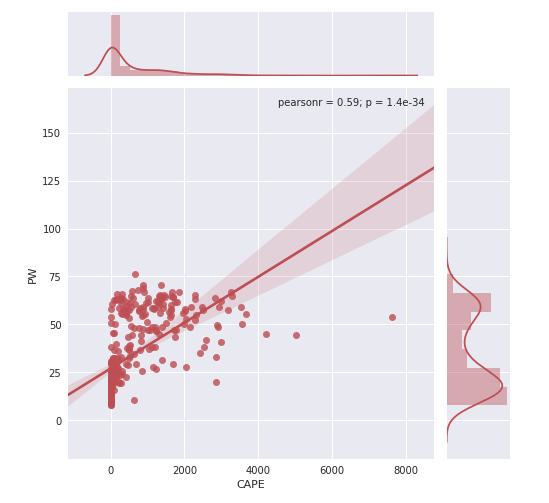
\includegraphics[width=0.3\textwidth]{7.png}
\caption{\label{fig:}Convective Available Potential Energy vs Agua Precipitable 12Z}
\end{figure}

\begin{figure}[h]
\centering
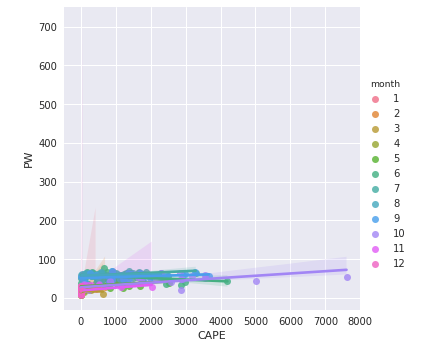
\includegraphics[width=0.3\textwidth]{8.png}
\caption{\label{fig:}Convective Available Potential Energy vs Agua Precipitable 12Z}
\end{figure}

\section{Conclusiones}

\subsection{00Z}

De la figura 1 podemos concluir que fue entre el quinto y el decimo mes que hubo inestabilidad en las parcelas de aire para 00z. En la figura 2, podemos observar como en estos meses fue donde hubo más agua precipitable. Por lo tanto podemos sospechar que exista una relacion.
\linebreak

De las figuras 3 y 4, sobre todo de la 3, podemos apreciar como existe una relacion lineal entre PW y CAPE.



\subsection{12Z}

De nuevo, se puede apreciar como CAPE tuvo su mayor presencia entre mayo y octubre, al ver la figura 5. De la figura 6, podemos notar que tambien fue entre mayo y cotubre donde el agua presipitab le tubo sus valores más altos, delatando una posible relacion.
\linebreak

utilizando las figuras 7 y 8, podemos apreciar como existe una relacion lienal entre PW y CAPE, y al haber sucedido en 12Z y 00Z podemos confirmar que esta existe.

\section{Bibliografia}

\begin{verbatim}


Wikipedia. (2016). Precipitable water. 6 de Marzo del 2018, de Wikipedia Sitio web: https://en.wikipedia.org/wiki/Precipitable_water

Wikipedia. (2018). Convective available potential energy. 6 de Marzo del 2018, de Wikipedia Sitio web: https://en.wikipedia.org/wiki/Convective_available_potential_energy

\end{verbatim}

\section{Apendice}

    ¿Cómo se te hizo esta actividad? ¿Compleja, Difícil, Sencilla?
    \linebreak
    Me parecio algo dificil, ya que al principio no tenia ni la más minima idea de como limpiar el archivo, ni que comandos usar.
    \linebreak
    ¿Qué te llamó más la atención?
    \linebreak
    Lo util que pueden ser ciertos elementos para limpiar un archivo para despues poderlo procesar.
    \linebreak
  
    ¿Qué parte fue la que menos te interesó hacer?
    \linebreak
    Escribir el reporte en Latex.
    \linebreak
    ¿Cómo mejorarías esta actividad? ¿Qué le faltó? ¿Qué sobró?
    \linebreak
    Vendria bien una introduccion.
    \linebreak
    ¿Hasta este punto, que te parece el uso de Jupyter para programar en Python?
    \linebreak
    Me aprece una herramienta muy util para procesar mucah informacion de forma rapida, aunque aun me resulta un poco desconocida e encriptada.


\end{document}